\section{Festigkeitslehre}
\subsection{Spannungen}
% E => G
\hrule
\begin{eeqn}{Umrechnung zwischen Schubmodul $G$ und Elastizitätsmodul $E$}
 		\begin{flalign}
 			G &= \frac{E}{2(1+\mu)}
		\end{flalign}
		Für Stähle gilt $\mu=0,33$
\end{eeqn}
\begin{figure}[H]
	\begin{minipage}[b]{0.22\linewidth}
		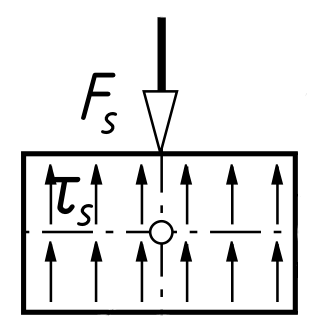
\includegraphics[width=\linewidth]{festigkeitslehre/scherung}
		\caption*{Scherspannungen}
	\end{minipage}
	\begin{minipage}[b]{0.5\linewidth}
		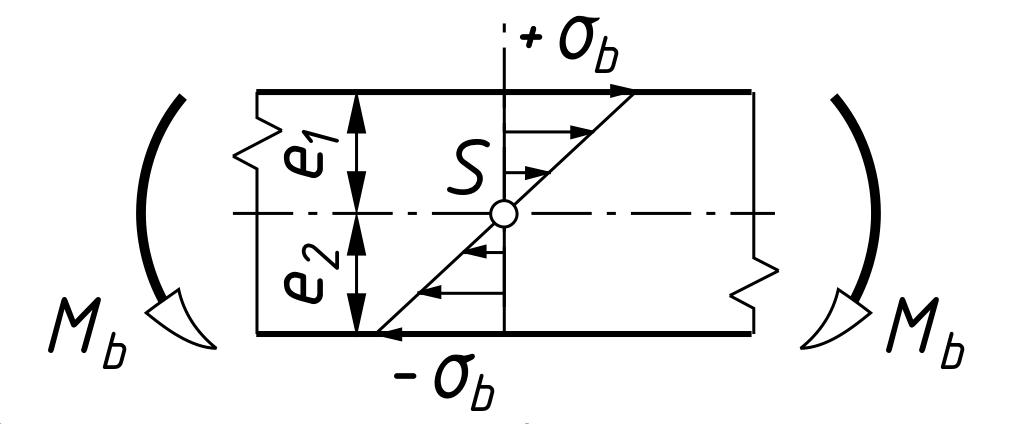
\includegraphics[width=\linewidth]{festigkeitslehre/biegung}
		\caption*{Biegespannungen}
	\end{minipage}
	\begin{minipage}[b]{0.26\linewidth}
		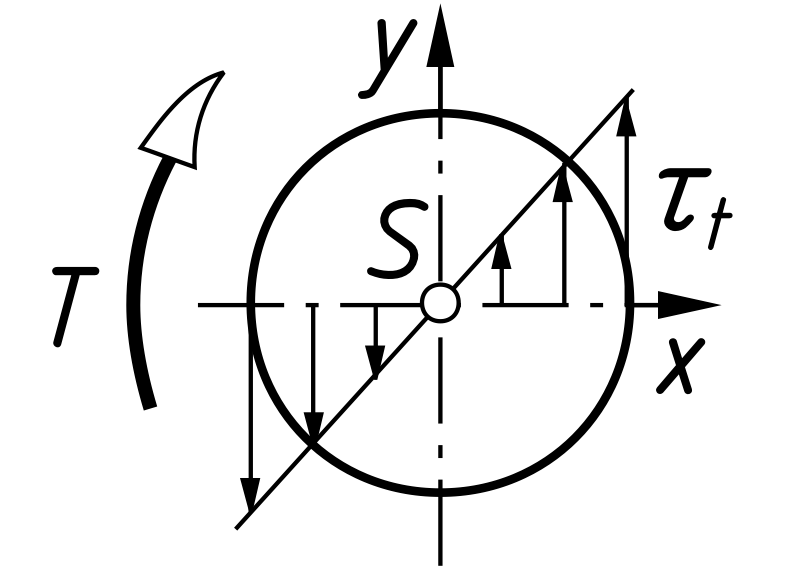
\includegraphics[width=\linewidth]{festigkeitslehre/torsion}
		\caption*{Torsionsspannungen}
	\end{minipage}
\end{figure}
% Biegespannungen
\hrule
\begin{eeqn}{Biegespannungen}
 		\begin{flalign}
 			\sigma_\text{B} & = \frac{M_\text{B}}{W_\text{ax}}
		\end{flalign}
\end{eeqn}
% Torsionsspannungen
\begin{eeqn}{Torsionsspannungen}
 		\begin{flalign}
 			\tau_\text{t} & = \frac{M_\text{t}}{W_\text{t}}
		\end{flalign}
		Für Kreis- und Rohrgeometrien ist $W_\text{t}=W_\text{p}$
\end{eeqn}
% Scherspannungen
\begin{eeqn}{Scherspannungen}
 		\begin{flalign}
 			\tau_\text{A} & = \frac{F_\text{A}}{A}
		\end{flalign}
\end{eeqn}

\subsection{Widerstandsmomente}
\begin{table}[H]
\begin{tabularx}{\linewidth}{m{30mm}XX}
	\toprule
	Geometrie & $I$ & $W$ \\
	\midrule
	% Kreis
	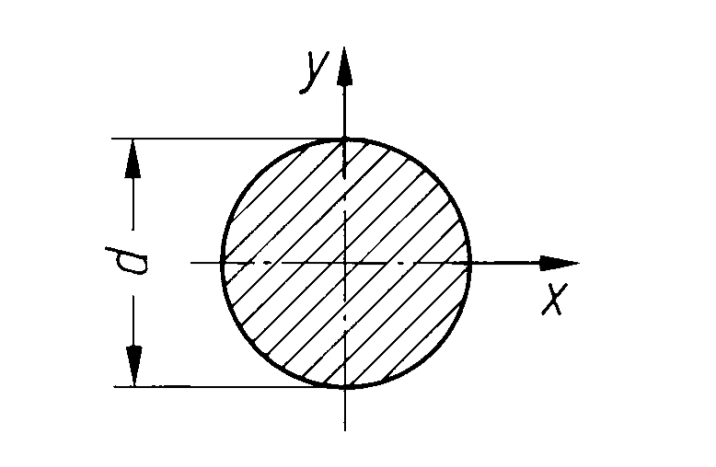
\includegraphics[width=30mm]{festigkeitslehre/kreis} & $\begin{aligned} & I_\text{ax} = \frac{\pi d^4}{64} \\ &I_\text{p} = \frac{\pi d^4}{32}\end{aligned}$ & $\begin{aligned} &W_\text{ax} = \frac{\pi d^3}{32} \\ &W_\text{p}=\frac{\pi d^3}{16}\end{aligned}$\\ \midrule
	% Kreisring
	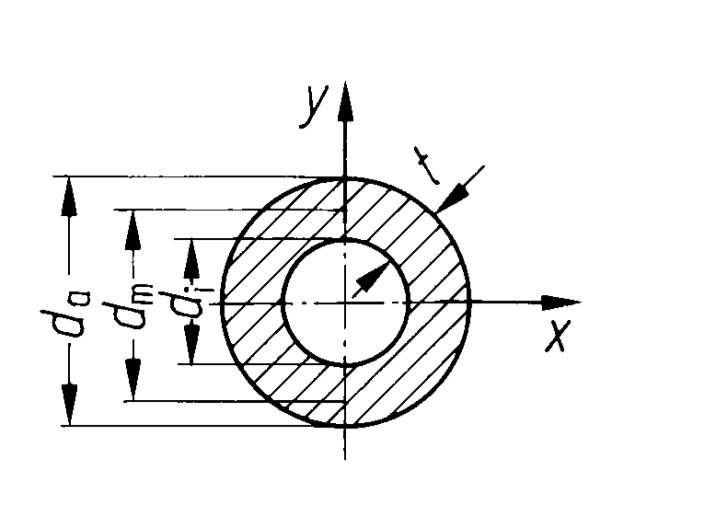
\includegraphics[width=30mm]{festigkeitslehre/kreisring} & $\begin{aligned} & I_\text{ax} = \frac{\pi (d_\text{a}^4-d_\text{i}^4)}{64} \\ &I_\text{p} = \frac{\pi (d_\text{a}^4-d_\text{i}^4)}{32}\end{aligned}$ & $\begin{aligned}& W_\text{ax} = \frac{\pi (d_\text{a}^4-d_\text{i}^4)}{32\cdot d_\text{a}} \\ &W_\text{p}=\frac{\pi (d_\text{a}^4-d_\text{i}^4)}{16\cdot d_\text{a}} \end{aligned}$\\ \midrule
	% Rechteck
	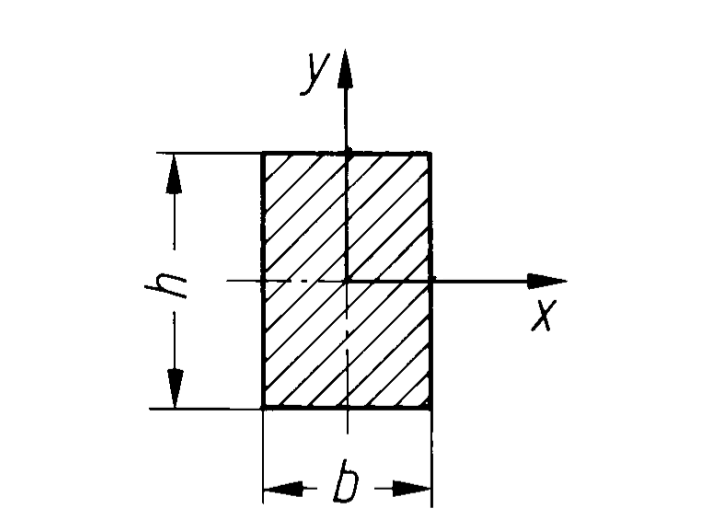
\includegraphics[width=30mm]{festigkeitslehre/rechteck} & $\begin{aligned} & I_\text{x} = \frac{bh^3}{12} \\ &I_\text{y} = \frac{b^3h}{12} \end{aligned}$ & $\begin{aligned} W_\text{x} = \frac{bh^2}{6} \\ W_\text{y} = \frac{b^2h}{6}\end{aligned}$ \\ \midrule
	% Quadrat
	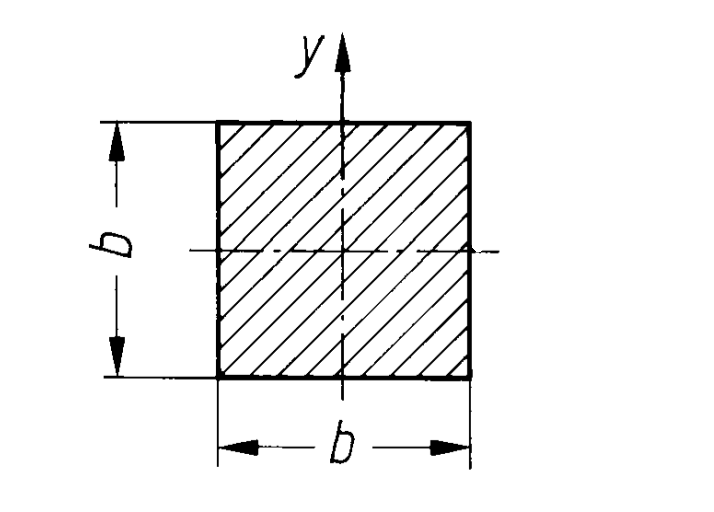
\includegraphics[width=30mm]{festigkeitslehre/quadrat} & $\begin{aligned} & I_\text{ax} = \frac{b^4}{12} \end{aligned}$ & $\begin{aligned} W_\text{ax} = \frac{b^3}{6} \end{aligned}$ \\ \midrule
	% Dreieck
	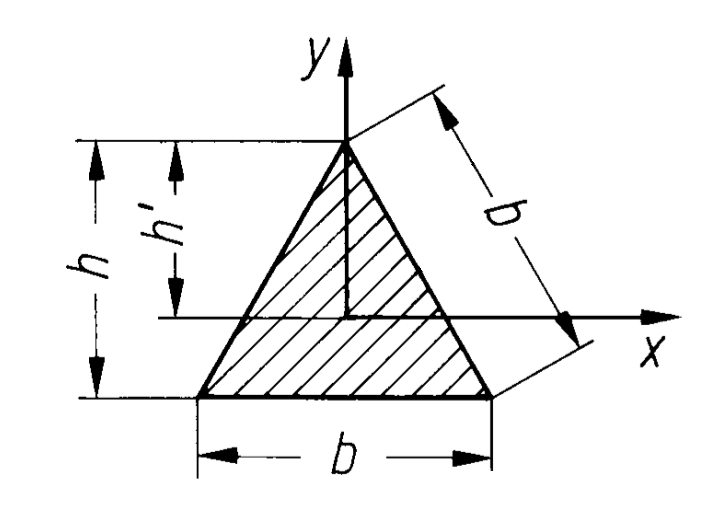
\includegraphics[width=30mm]{festigkeitslehre/dreieck} & $\begin{aligned} & I_\text{x} = \frac{bh^3}{36} \\ &I_\text{y} = \frac{b^3h}{48} \end{aligned}$ & $\begin{aligned} W_\text{x} = \frac{bh^2}{24} \\ W_\text{y} = \frac{b^2h}{24}\end{aligned}$ \\\bottomrule
\end{tabularx}
\end{table}
\vfill
\pagebreak

\subsection{Mohr'scher Spannungskreis}
\begin{figure}[H]
	\centering
	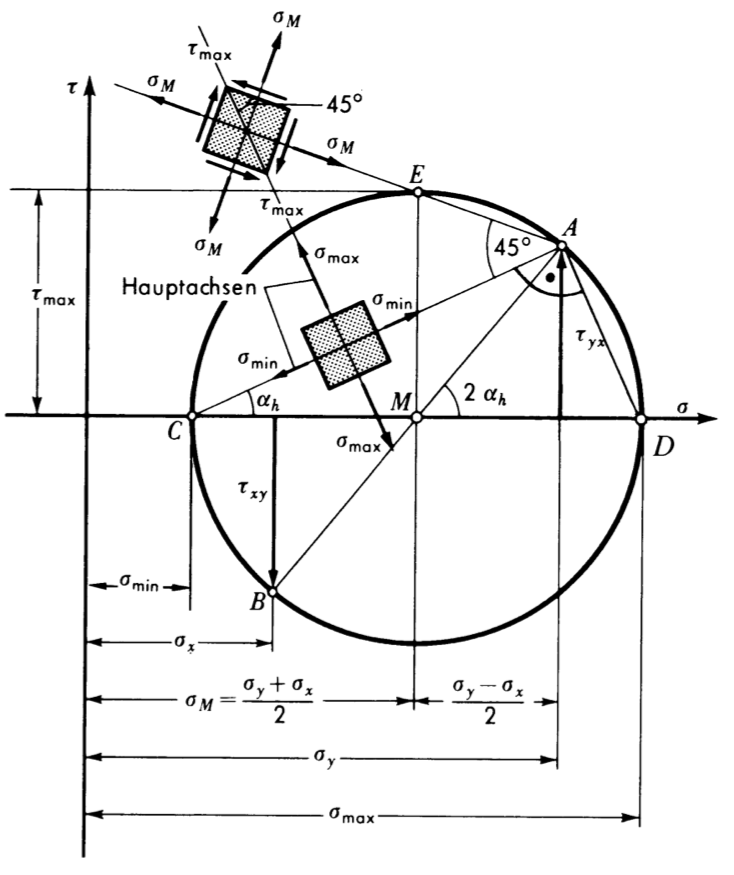
\includegraphics[width=0.63\linewidth]{festigkeitslehre/mohrischer-spannungskreis}
	\caption*{Mohrischer Spannungskreis}
\end{figure}

% maximale Spannungen
\hrule
\begin{eeqn}{max/min Spannnungen}
	\begin{flalign}
		\sigma_{1,2} & = \frac{\sigma_\text{x}+\sigma_\text{y}}{2} \pm \frac{1}{2} \sqrt{(\sigma_\text{x}-\sigma_\text{y})^2+4\tau_\text{xy}^2} 
	\end{flalign}
	Im Mohr'schem Spannungskreis befinden sich diese Spannungen bei den Nullstellen auf der Spannungsachse, auch Hauptspannungen genannt.
\end{eeqn}

% Winkel
\begin{eeqn}{gedrehte Spannungen}
	\begin{flalign}
		\tan 2\alpha & = \frac{2\tau_\text{xy}}{\sigma_\text{x}-\sigma_\text{y}}
	\end{flalign}
	Der Winkel $\alpha$ gibt an, um wie viel Grad das Koordinatensystem gedreht wird. Setzt man $\tau_\text{xy} = 0$, erhält man den Winkel unter dem die Hauptspannungen auftreten. 
\end{eeqn}

\subsection{Vergleichs\-spannungs\-hypothesen}
% NSH
\hrule
\begin{eeqn}{Normalspannungs\-hypothese (NSH)}
	\begin{flalign}
		\sigma_\text{v} & = \frac{\abs{\sigma_\text{x}+\sigma_\text{y}}}{2} + \frac{1}{2} \sqrt{(\sigma_\text{x}-\sigma_\text{y})^2+4\tau_\text{xy}^2}
	\end{flalign}
	Die Vergleichsspannung $\sigma_\text{v}$ entspricht der maximalen Normalspannung.
\end{eeqn}

% SSH
\begin{eeqn}{Schubspannungs\-hypothese (SSH)}
	\begin{align}
		&\sigma_1 > \sigma_2 > 0: &\quad \sigma_\text{v} &= \sigma_1 \\
		& \sigma_1 > 0 > \sigma_2: &\quad  \sigma_\text{v}& = \sigma_1 - \sigma_2 \\
		& 0 > \sigma_1 > \sigma_2: &\quad \sigma_\text{v} &= \abs{\sigma_2}
	\end{align}
	Die Vergleichsspannung $\sigma_\text{v}$ entspricht der maximalen Schubspannung.
\end{eeqn}

% GEH
\begin{eeqn}{Gestaltänderungs\-hypothese (GEH)}
	\begin{flalign}
		\sigma_\text{v} &= \sqrt{\sigma_{x}^2+\sigma_{y}^2-\sigma_{x}\sigma_{y}+3\tau_\text{xy}^2}
	\end{flalign}
	Diese Formel entspricht einem zweiachsigen Spannungszustand. Für mehrachsige Spannungszustände siehe Skript. I.d.R: $\tau_\text{xy}^2 = \tau_\text{A}^2+ \tau_\text{t}^2$
\end{eeqn}
\vfill
\pagebreak


\subsection{Dauerfestigkeit}
\begin{vardef}
	\item[$\beta_\text{k}$] Kerbwirkungsfaktor
	\item[$b_1$] Oberflächenbeiwert (siehe Diagramm: ad gegen $R_\text{m}$)
	\item[$b_2$] Größenbeiwert (siehe Diagramm: Wellendruchmesser)
	\item[$\sigma_\text{z, sch}$] Maximal auftretende Spannungen bei reiner Zugschwellbelastung
	\item[$\sigma_\text{gak}$] Ausschlagsspannung unter Berücksichtigung von Gestalt und Kerbwirkung
	\item[$\sigma_\text{gk,zdw}$] Zug- Druck Wechselspannung unter Berücksichtigung von Gestalt und Kerbwirkung 
\end{vardef}

\begin{figure}[H]
	\centering
	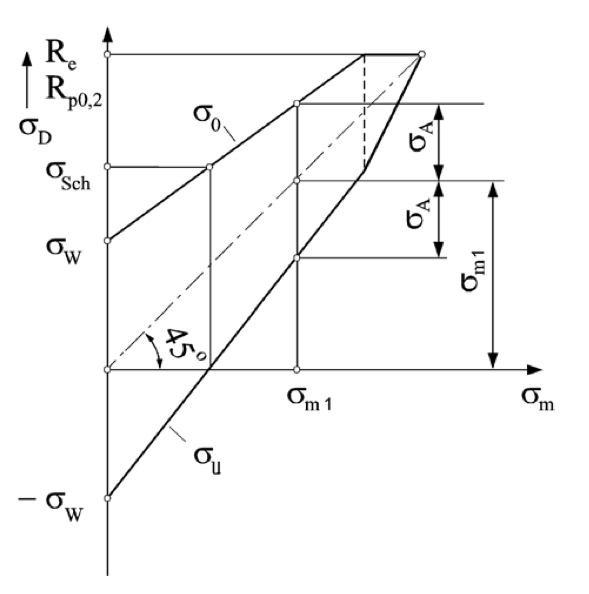
\includegraphics[width=0.5\linewidth]{festigkeitslehre/smith-diagramm}
	\caption*{Dauerfestigkeitsdiagramm nach Smith}
\end{figure}

\hrule
% 1. Reduktion
\begin{eeqn}{1. Reduktion}
	\begin{flalign}
		& \sigma_\text{z, zul}^* = R_\text{e} \cdot b_2 \\
		& \sigma_\text{zdw}^* = \sigma_\text{zdw} \cdot b_2\\
		& \sigma_\text{z, sch}^* = \sigma_\text{z, sch} \cdot b_2 \\
		& \sigma_\text{a}^* = \sigma_\text{a} \cdot b_2
	\end{flalign}
\end{eeqn}
\begin{eeqn}{2. Reduktion}
	\begin{flalign}
		& K = \frac{b_1}{\beta_\text{k}}\\
		& \sigma_\text{gak} = \sigma_\text{a}^*\cdot K \\
		& \sigma_\text{gzdw} = \sigma_\text{zdw}^* \cdot K
	\end{flalign}
\end{eeqn}
